%----------------------------------------------------------------------------
\chapter{Unit Testing in LabVIEW}
\label{chap:testing}
%----------------------------------------------------------------------------

Unit testing in LabVIEW programs are commonly used in medium or large size projects, or where requirements are changing. Though, it is not a common practice everywhere, even if the project is an industrial application, where a fault is really expensive to recover. The main reason is to cut testing costs.

The testing techniques are similar to those in traditional programming languages, with a few differences. Software units can be a single VI, a group of VIs, or a LabVIEW class. Unit tests follow the xUnit schema: the tested unit gets pre-defined input sets, and the results are compared to the pre-defined outputs.

It is important to write testable code, that can run isolated from external dependencies, and does not require to run the entire program. "Spaghetti code", that is not able to run on its own, is not only bad from the perspective of testing, but can cause other problems (like re-usability in other projects, or maintaining compatibility with new versions of other components). In LabVIEW, it is really easy to fall in this trap, but following development guidelines help to evade it. Following Test Driven Development is also possible in LabVIEW, with nearly the same rules as in other languages - when the interface of a unit is defined, creating tests can begin \cite{delacor_ni2014}. 

\section{Self-made test fixtures}
It is always an option to build a test fixture manually (and in NXG it is the only option currently). Every test suite will get a harness VI, which executes several test cases. Test cases of a test suite will do the same action on the unit, but with several different input sets. The inputs and expected outputs can be defined in an array, a cluster, or other data structure, and then a loop iterates over the test cases, executing the VI under test for each set of parameters. The test verifies output values and error output if it is present. Setup and teardown parts can be included in the loop too (or global setup and teardown outside the loop), to initialize and prepare the unit, and to do any clean-up task necessary. A boolean output will indicate, whether the test suite passed or failed - in order to pass, all test cases must pass. The block diagram of an example test fixture is shown on Figure~\ref{fig:selfmadetestfixture}.
A top module is recommended, which contains all the Harness VIs, and summarizes the results. This could substitute the interface of a unit testing framework. 

\begin{figure}
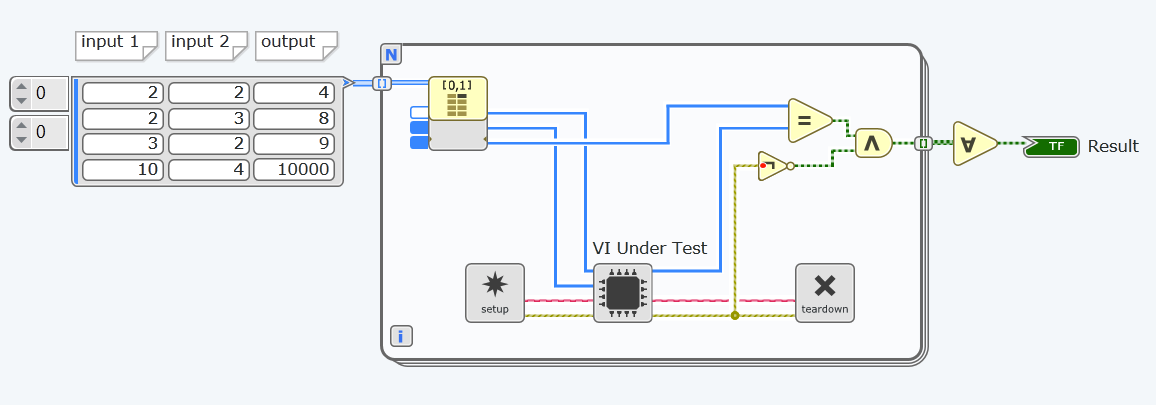
\includegraphics[width=150mm,keepaspectratio]{figures/lv_testsuite.png}
\caption{A test fixture in LabVIEW NXG} 
\label{fig:selfmadetestfixture}
\end{figure}

\section{Testing frameworks}

There are really few unit testing tools and frameworks for LabVIEW compared to other languages\footnote{\url{https://en.wikipedia.org/wiki/List_of_unit_testing_frameworks}}, and they only support current generation LabVIEW (LV 2018), and not NXG.

\paragraph{Unit Test Framework}
Unit Test Framework\footnote{\url{http://sine.ni.com/nips/cds/view/p/lang/hu/nid/209043}} (or UTF for short) is the official unit testing tool for LabVIEW, released by National Instruments. It is available for purchase as an addon from LabVIEW Tools Network. UTF is the most popular unit testing framework, since it is covered by the support of National Instruments, an ISO certified company.

The interface of UTF is really easy to use, a unit test can be made in a few minutes. Test suites are stored in .lvtest files, which can be edited with a configuration panel. A tabular-style interface is used to define the inputs and outputs for each test case. Setup and teardown VIs, and other options can also be defined. There are a few special cases, when the desired behaviour cannot be expressed using the editor (like passing parameters to a teardown VI).

The results are shown in a dialog with other metrics, like code coverage. Status of the tests are shown also in the Project Explorer, for a quick check. UTF has the advantage to run tests on real-time NI hardware, like the CompactRIO\footnote{\url{http://www.ni.com/en-us/shop/compactrio.html}} \cite{labview_utf}. 
\paragraph{JKI VI Tester}
VI Tester\footnote{\url{http://sine.ni.com/nips/cds/view/p/lang/hu/nid/215910}} is an open source tool from JKI Software. Based on the xUnit test achitecture, it is a really powerful test framework, that supports testing object-oriented LabVIEW programs well. Tests are created from a template, and organized into a test class. Assertion and other utilities can be used as a testing element subVI, as seen on Figure \ref{fig:vitester}. \cite{vitesterwiki}
\begin{figure}
\centering
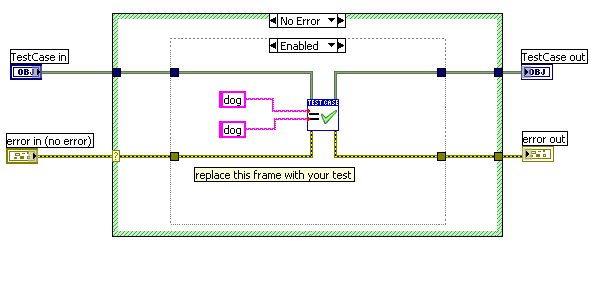
\includegraphics[width=120mm,keepaspectratio]{figures/vitester.png}
\caption{Example VI with an assertion} 
\label{fig:vitester}
\end{figure}
\paragraph{Caraya}
Another unit test framework from JKI Software is Caraya\footnote{\url{http://sine.ni.com/nips/cds/view/p/lang/hu/nid/215909}}, which uses a different approach. The main feature is the assertion subVI, which can be used on its own (outside a unit test), to ensure validity of data in a system in production. Tests are defined with Test Suite and Define Test subVIs, and unit tests defined like that get summarized in an interface like in JKI VI Tester \cite{carayapages}. 
\paragraph{InstaCoverage}
InstaCoverage\footnote{\url{http://sine.ni.com/nips/cds/view/p/lang/hu/nid/216652}} is a new, xUnit-style tool. The test suites are stored in a similar way to UTF, but each test gets a harness VI, like in JKI's tools. Harness VIs are really minimalistic, therefore test execution is really quick. InstaCoverage tests can also run on real-time hardware \cite{icovsite}. 
\section{Conclusion}
The presented tools are good in executing unit tests an summarizing the results of testing. They also provide a test skeleton template or a UI to help create unit tests, but it is still quite complicated and takes time to build a test suite for either framework. Lots of developers choose not to create unit tests, even for industrial projects, to spare time or cut costs. The tool I am planning to implement can be the part of a solution, which can make unit test creation an automatic process, making it a minimal overhead to developers (like, e.g. IntelliTest).   